% 
% Annual CCN conference
% Sample LaTeX Two-Page Summary -- Proceedings Format
% based on the prior cognitive science style file

% Original : Ashwin Ram (ashwin@cc.gatech.edu)       04/01/1994
% Modified : Johanna Moore (jmoore@cs.pitt.edu)      03/17/1995
% Modified : David Noelle (noelle@ucsd.edu)          03/15/1996
% Modified : Pat Langley (langley@cs.stanford.edu)   01/26/1997
% Latex2e corrections by Ramin Charles Nakisa        01/28/1997 
% Modified : Tina Eliassi-Rad (eliassi@cs.wisc.edu)  01/31/1998
% Modified : Trisha Yannuzzi (trisha@ircs.upenn.edu) 12/28/1999 (in process)
% Modified : Mary Ellen Foster (M.E.Foster@ed.ac.uk) 12/11/2000
% Modified : Ken Forbus                              01/23/2004
% Modified : Eli M. Silk (esilk@pitt.edu)            05/24/2005
% Modified : Niels Taatgen (taatgen@cmu.edu)        10/24/2006
% Modified : David Noelle (dnoelle@ucmerced.edu)     11/19/2014
% Modified : Konrad Kording (koerding@gmail.com) 2/15/2017

%% Change "letterpaper" in the following line to "a4paper" if you must. 
% Alternatively, just ignore that because who prints papers anymore?

\documentclass[10pt,letterpaper]{article}

\usepackage{ccn}
\usepackage{pslatex}
\usepackage{apacite}
\usepackage{graphicx}


\title{Neural Correlates of Context Function in Associative Learning}
 
\author{{\large \bf Samuel Gershman (gershman@fas.harvard.edu)} 
  \AND {\large \bf Momchil Tomov (mtomov@g.harvard.edu)} 
  \AND {\large \bf Hayley Dorfman (hdorfman@g.harvard.edu)} \\ \\
  Department of Psychology and Center for Brain Science,\\
  Harvard University, 52 Oxford St., room 295.05\\
Cambridge, MA 02138, USA}


\begin{document}

\maketitle


\begin{quote}
\small
\textbf{Keywords:} 
Bayesian modeling; Animal and human associative learning; Context-dependent learning
\end{quote}

\section{Introduction}



\section{Materials and Methods}

\subsubsection{Subjects.}

We recruited 28 healthy subjects (X female; Y-Z years of age; mean age Z +- SEM) to participate in this study. Eight participants were excluded due to excessive motion or insufficient data. The study was approved by the Harvard Institutional Review Board (IRB).

\begin{figure}[ht]
\begin{center}
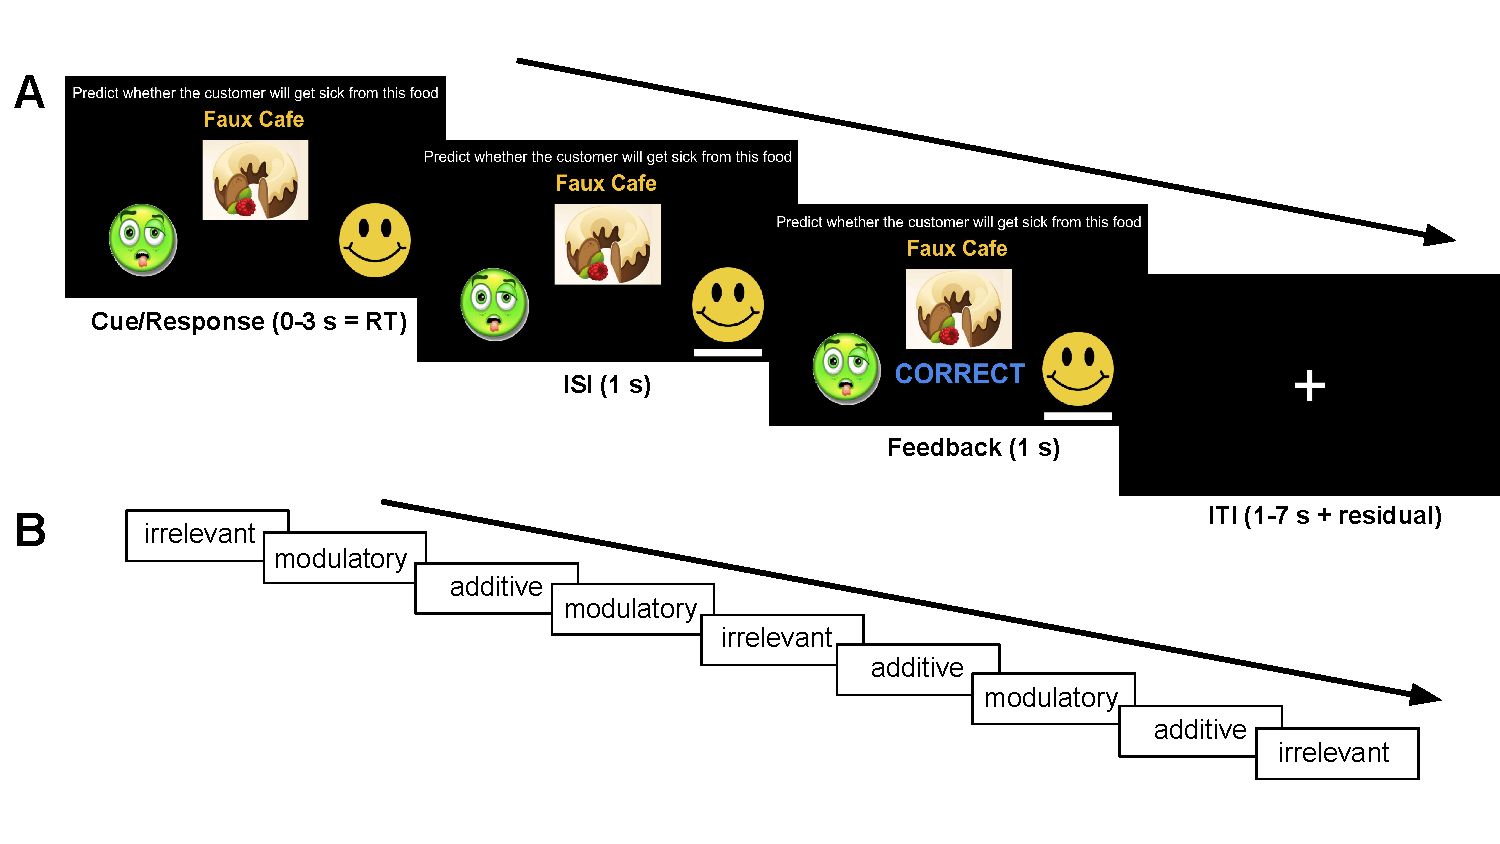
\includegraphics[width=0.5\textwidth]{task-design.pdf}
\end{center}
\vspace{-1em}
\caption{Experimental design. (A) Example timeline of events during a training trial. (B) Example sequence of blocks with the corresponding condition for each block. } 
\label{task-design}
\end{figure}

\subsubsection{Experimental design.} 

We adapted the task used in \citeA{Gershman2017} with a mixed within-subjects design consisting of 9 blocks. Each block consisted of 20 training trials followed by 4 test trials. On each training trial, participants were asked to predict whether a particular food (the cue) in a particular restaurant (the context) would cause sickness (the outcome) and were subsequently informed whether their prediction was correct (Figure~\ref{task-design}A). On each test trial, participants were asked to make a prediction about an old or a novel cue in an old or a novel context, without receiving any feedback, with each of the 2x2 combinations appearing exactly once. In each block, the cue-outcome contingencies depended on the context in accordance with one of the three causal interpretations which we refer to as the condition for that block. The nine blocks were divided in three consecutive groups such that each condition appeared in exactly one block in each group (Figure~\ref{task-design}B). Thus each participant learned under each condition three times. Each block contained a different set of foods and restaurants that were randomized across blocks.
\\

\subsubsection{Simulations.} 

We implemented the model presented in \citeA{Gershman2017}. The model had two free parameters: the variance $\sigma^2_w$ of the Gaussian prior from which the weights are assumed to be drawn; and the inverse temperature $\beta$ used in the logistic transformation from predictive posterior expectation to choice probability. Intuitively, the former corresponds to the level of uncertainty in the initial estimate of the weights, while the latter reflects the exploration-exploitation tradeoff of the model choices. We fit these parameters using maximum likelihood parameter estimation based on behavioral data obtained from 10 different subjects who performed the same task outside the scanner during a pilot version of the study (data not shown). The fitted values were $\sigma^2_w = 0.1249$ and $\beta = 2.0064$. All other parameters had the same values as described in \citeA{Gershman2017}. Each block was simulated independently using the same set of parameters.


\section{Results}

\begin{figure}[ht]
\begin{center}
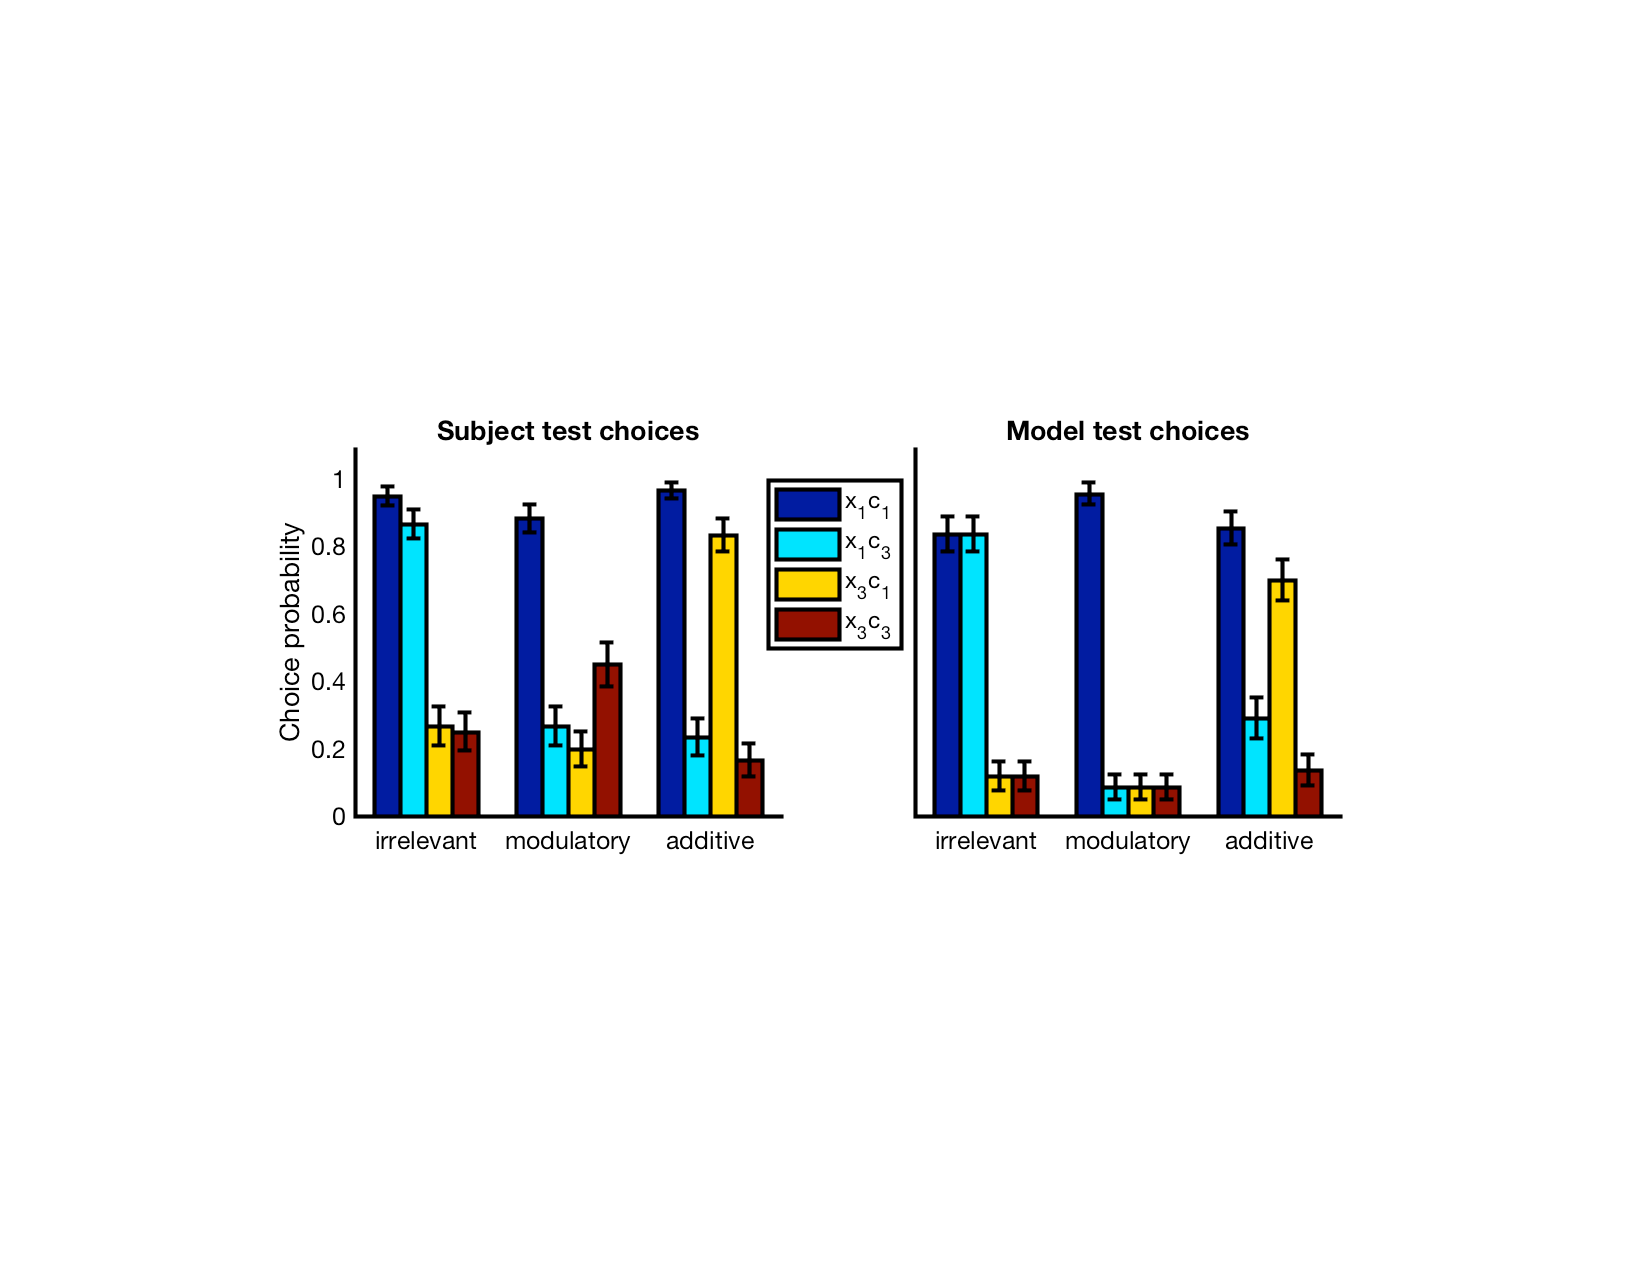
\includegraphics[scale=0.45,  trim = 120 220 120 200]{behavioral.pdf}
\end{center}
\caption{Subject (left) and model (right) performance on the test trials.} 
\label{behavioral}
\end{figure}

\subsubsection{Behavioral performance.}

Test trial choices averaged across blocks are shown in Figure~\ref{behavioral}. Overall, participants learned the task quickly and exhibited the same within-subjects behavioral pattern as was previously reported using a between-subjects design \cite{Gershman2017}. The model successfully accounted for participants' choices on both the training and the test trials ($r = 0.7283, p < 0.00001$) using the parameters obtained from pilot data from a different set of participants.

\begin{figure}[ht]
\begin{center}
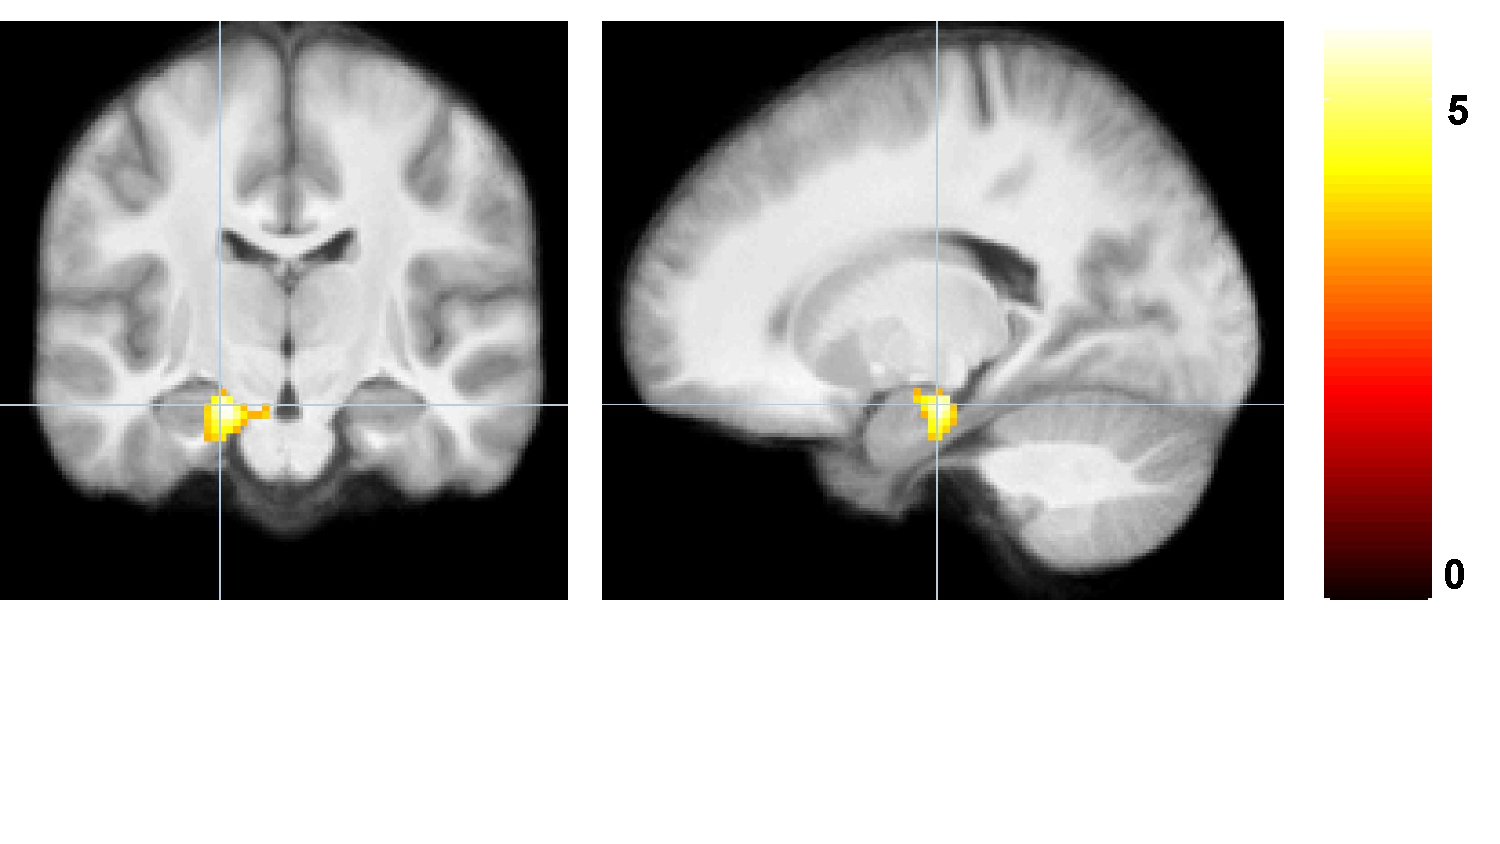
\includegraphics[scale=0.33,  trim = 0 150 0 0]{additive-irrelevant.pdf}
\end{center}
\caption{Transient activity related to the additive condition minus the irrelevant condition in left anterior hippocampus (MNI: -18 -16 -18, $t > 3.5518, p < 0.001$, cluster FWE corr). Right: T-value scale.} 
\label{additive-irrelevant}
\end{figure}

\subsubsection{Imaging data.} 

We had an a priori hypothesis that the hippocampus would be involved in modulating the cue-outcome association when it is influenced by the context. We therefore contrasted BOLD activation between blocks in the different conditions at the time of outcome presentation during the training phase. The BOLD signal did not differ significantly between the modulatory and the irrelevant conditions, nor between the modulatory and the additive conditions. The contrast between the additive and the irrelevant conditions showed increased activation in left anterior hippocampus (Figure~\ref{additive-irrelevant}; MNI coordinates of peak voxel: [-18 -16 -18]; t-value: 5.748; extent with $t > 3.5518$: 141; $p < 0.001$; cluster FWE corrected). Each contrast also included a constant regressor at the time of trial onset to account for the visual activation.

In order to measure the neural correlates of structure learning, we computed a contrast with a parametric modulator corresponding to the Kullback--Leibler divergence of the posterior over causal structures which is updated by the model at the time of outcome presentation on each training trial. The results are shown in Table~\ref{kl-divergence-table} and Figure TODO. We found significant bilateral activation in the parietal cortex (the angular gyri), rostrolateral prefrontal cortex (rlPFC). 

\begin{table}[!ht]
\begin{center} 
\caption{Brain activation tracking the Kullback--Leibler divergence of the posterior over causal structures during training. Only cerebral regions with T-value $ > 5$ are shown. All P-values are $< 0.001$ with cluster FWE correction. Regions were automatically labeled using the AAL2 atlas.} 
\label{kl-divergence-table} 
\vskip 0.12in
\begin{tabular}{llll} 
\hline
Brain region    &  Extent & T-value  & MNI coordinates \\
\hline
Angular (R) &	484	& 8.638 &	34	-64	48\\
Frontal Inf Oper (R) &	341 &	8.378& 48	20	34 \\
Frontal Mid 2 (R) &	130	& 7.440 &	36	56	-2 \\
Frontal Mid 2 (L) &	173	& 7.205 &	-42	56	2 \\
Frontal Mid 2 (R) &	86	& 6.996 &	34	12	54 \\
Parietal Inf (L) &	254 	& 6.699 &	-30	-54	42 \\
Parietal Sup (L)	 & 254	& 5.566 &	-34	-72	54 \\
Frontal Inf Tri (L) &	173	& 6.583 & -44	20	22 \\
Temporal Inf (R) &	 15	& 6.461 &	60	-24	-20 \\
Insula (L)	& 18	 & 6.272	& -28	22	-2 \\
OFCant (R)& 	8  &	5.827 &	20	48	-16 \\
\hline
\end{tabular} 
\end{center} 
\end{table}





\section{General Formatting Instructions}

The entire contribution of a short summary submission (including
figures, references, and anything else) can be no longer than two
pages. This short summary format is to be used for workshop and
tutorial descriptions, symposia summaries, and publication-based
presentation extended abstracts. Unlike submitted research papers,
short summary submissions should \emph{not} begin with a separate
abstract. Prior to the first section of the short summary, there
should be the header ``{\bf Keywords:}'' followed by a list of
descriptive keywords separated by semicolons, all in 9~point font, as
shown above.

The text of the paper should be formatted in two columns with an
overall width of 7 inches (17.8 cm) and length of 9.25 inches (23.5
cm), with 0.25 inches between the columns. Leave two line spaces
between the last author listed and the text of the paper. The left
margin should be 0.75 inches and the top margin should be 1 inch.
\textbf{The right and bottom margins will depend on whether you use
  U.S. letter or A4 paper, so you must be sure to measure the width of
  the printed text.} Use 10~point Modern with 12~point vertical
spacing, unless otherwise specified.

The title should be in 14~point, bold, and centered. The title should
be formatted with initial caps (the first letter of content words
capitalized and the rest lower case). Each author's name should appear
on a separate line, 11~point bold, and centered, with the author's
email address in parentheses. Under each author's name list the
author's affiliation and postal address in ordinary 10~point type.

Indent the first line of each paragraph by 1/8~inch (except for the
first paragraph of a new section). Do not add extra vertical space
between paragraphs.


\section{First Level Headings}

First level headings should be in 12~point, initial caps, bold and
centered. Leave one line space above the heading and 1/4~line space
below the heading.


\subsection{Second Level Headings}

Second level headings should be 11~point, initial caps, bold, and
flush left. Leave one line space above the heading and 1/4~line
space below the heading.


\subsubsection{Third Level Headings}

Third level headings should be 10~point, initial caps, bold, and flush
left. Leave one line space above the heading, but no space after the
heading.


\section{Formalities, Footnotes, and Floats}

Use standard APA citation format. Citations within the text should
include the author's last name and year. If the authors' names are
included in the sentence, place only the year in parentheses, and
\citeA{NewellSimon1972a}, but otherwise place the entire reference in
parentheses with the authors and year separated by a comma
\cite{NewellSimon1972a}. List multiple references alphabetically and
separate them by semicolons
\cite{ChalnickBillman1988a,NewellSimon1972a}. Use the
``et~al.'' construction only after listing all the authors to a
publication in an earlier reference and for citations with four or
more authors.


\subsection{Footnotes}

Indicate footnotes with a number\footnote{Sample of the first
footnote.} in the text. Place the footnotes in 9~point type at the
bottom of the column on which they appear. Precede the footnote block
with a horizontal rule.\footnote{Sample of the second footnote.}


\subsection{Tables}

Number tables consecutively. Place the table number and title (in
10~point) above the table with one line space above the caption and
one line space below it, as in Table~\ref{sample-table}. You may float
tables to the top or bottom of a column, or set wide tables across
both columns.

\begin{table}[!ht]
\begin{center} 
\caption{Sample table title.} 
\label{sample-table} 
\vskip 0.12in
\begin{tabular}{ll} 
\hline
Error type    &  Example \\
\hline
Take smaller        &   63 - 44 = 21 \\
Always borrow~~~~   &   96 - 42 = 34 \\
0 - N = N           &   70 - 47 = 37 \\
0 - N = 0           &   70 - 47 = 30 \\
\hline
\end{tabular} 
\end{center} 
\end{table}


\subsection{Figures}

Make sure that the artwork can be printed well (e.g. dark colors) and that 
the figures make understanding the paper easy.
 Number figures sequentially, placing the figure
number and caption, in 10~point, after the figure with one line space
above the caption and one line space below it, as in
Figure~\ref{sample-figure}. If necessary, leave extra white space at
the bottom of the page to avoid splitting the figure and figure
caption. You may float figures to the top or bottom of a column, or
set wide figures across both columns.

\section{Acknowledgments}

Place acknowledgments (including funding information) in a section at
the end of the paper.


\section{References Instructions}

Follow the APA Publication Manual for citation format, both within the
text and in the reference list, with the following exceptions: (a) do
not cite the page numbers of any book, including chapters in edited
volumes; (b) use the same format for unpublished references as for
published ones. Alphabetize references by the surnames of the authors,
with single author entries preceding multiple author entries. Order
references by the same authors by the year of publication, with the
earliest first.

Use a first level section heading, ``{\bf References}'', as shown
below. Use a hanging indent style, with the first line of the
reference flush against the left margin and subsequent lines indented
by 1/8~inch. Below are example references for a conference paper, book
chapter, journal article, dissertation, book, technical report, and
edited volume, respectively.

\nocite{ChalnickBillman1988a}
\nocite{Feigenbaum1963a}
\nocite{Hill1983a}
\nocite{OhlssonLangley1985a}
% \nocite{Lewis1978a}
\nocite{Matlock2001}
\nocite{NewellSimon1972a}
\nocite{ShragerLangley1990a}


\bibliographystyle{apacite}

\setlength{\bibleftmargin}{.125in}
\setlength{\bibindent}{-\bibleftmargin}

\bibliography{ccn_style.bib}


\end{document}
